\documentclass{article}
\usepackage{graphicx} % Required for inserting images

\title{Digital Control Systems Coursework: Omar Ben-Gacem}
\author{Omar Ben-Gacem}
\date{January 2025}



%%%%%%%%%%%%     Formatting     %%%%%%%%%%%%

\usepackage[sorting=none]{biblatex} %Imports biblatex package

\addbibresource{bibliography.bib} %Import the bibliography file
\usepackage[margin=1in,headsep=.5in]{geometry}
\usepackage{amsmath} % for bmatrix and pmatrix
\usepackage{amssymb}
\usepackage{wrapfig}
\usepackage{caption}
\usepackage{fancyhdr}
\usepackage{subcaption}
\usepackage{gensymb}
\usepackage{float}
\usepackage{ragged2e}
\usepackage{booktabs} % For better table formatting
\usepackage[export]{adjustbox}
\geometry{
 a4paper,
 total={170mm,257mm},
 left=19mm,
 right=19mm,
 top=23mm,
 bottom=23mm
 }
\renewcommand{\sectionmark}[1]{%
    \markright{\MakeUppercase{#1}}%
}



\title{Digital Control Systems Coursework Submission}
\author{Omar Ben-Gacem}
\pagestyle{fancy}
\fancyhead[RO]{{\rightmark}}
\date{November 2024}
\lhead{Omar Ben-Gacem\\01883771\\Digital Control Systems Coursework}






%%%%%%%%%%%%     Formatting     %%%%%%%%%%%%


\begin{document}


% \section*{Executive Summary}
% \begin{equation}
R = \left(\begin{array}{cccc} 0 & \frac{1}{M} & -\frac{F}{M^2} & \frac{F^2}{M^3}\\ \frac{1}{M} & -\frac{F}{M^2} & \frac{F^2}{M^3} & -\frac{F^3}{M^4}\\ 0 & -\frac{1}{L\,M} & \frac{F}{L\,M^2} & -\frac{g}{L^2\,M}-\frac{F^2}{L\,M^3}\\ -\frac{1}{L\,M} & \frac{F}{L\,M^2} & -\frac{g}{L^2\,M}-\frac{F^2}{L\,M^3} & \frac{\frac{F^3}{L\,M^3}+\frac{F\,g}{L^2\,M}}{M} \end{array}\right)
\end{equation}



\section{System Dynamics (Part A)}
The system being modeled is an inverted pendulum attached to a sliding cart. The target is to control the liner displacement of the card in order to hold the pendulum in an inverted position. Equation \ref{eqofm} gives the Newtonian equations of motion for the cart-pendulum system.

\[
\begin{cases}
  M \ddot{s}(t) + F \dot{s}(t) - \mu(t) & = 0 \\
    \ddot{\phi}(t) - \frac{g}{L} \ddot{s}(t) \sin({\phi}(t)) - \frac{\mu(t)}{L} \cos(\phi(t)) & = 0
\end{cases}
\]

\subsection*{A1) Standard Form}
To write the cart-pendulum system in standard form, the state variable $\underline{x}$ and the input $\underline{u}$ must be identified. The applied force $\mu(t)$ acts as the only input to this system. By inspection of the equations of motion, it is trivial to show that displacement $s$ and angle $\phi$ both have first- and second-order differential terms, thus making state variable $\underline{x} = [s, \dot s, \phi, \dot\phi]^T$. Equation \ref{eqofm} can be rearranged and reduced to give Equation \ref{fofx} which acts as the state update function.

\begin{equation}\label{fofx}
    \dot{x}=\begin{bmatrix}\dot{s} \\ \ddot{s} \\ \dot{\phi} \\ \ddot{\phi}\end{bmatrix} = f(\underline{x},\underline{u}) = \n\left(\begin{array}{cccc} 0 & 1 & 0 & 0\\ 0 & -\frac{F}{M} & 0 & 0\\ 0 & 0 & 0 & 1\\ 0 & \frac{F}{LM} & \frac{g}{L} & 0 \end{array}\right)
\n \begin{bmatrix} s \\ \dot{s} \\ \phi \\ \dot{\phi}\end{bmatrix} +     \begin{bmatrix}
        0 \\
        \frac{1}{M} \\
        0 \\
        -\frac{1}{L M}
    \end{bmatrix}\,\mu(t)
\end{equation}

\subsection*{A2) Free Response Equilibrium}
Setting $u=\mu(t)=0$ gives the free response of the system, where the equilibrium of this system are values of $\underline{\dot x}=\underline{0}$. The values of $\underline{x}$ that satisfy this criteria are shown below in Equation \ref{ueqzero}.

\begin{equation}\label{ueqzero}
\begin{bmatrix}
    \dot s \\ \ddot s \\ \dot \phi \\ \ddot \phi
\end{bmatrix} =  \begin{bmatrix}
    0 \\ 0 \\ 0 \\ 0
\end{bmatrix} = \begin{bmatrix}
    \dot{s} \\
    \frac{u}{M}-\frac{F\dot{s}}{M}  \\
    \dot{\phi} \\
     \frac{g\sin\left(\phi \right)}{L}-\frac{u\cos\left(\phi \right)}{LM}+\frac{F\dot{s}\cos\left(\phi \right)}{LM} \\
\end{bmatrix} \rightarrow \mu=0 \rightarrow \underline{x} = \begin{bmatrix}
    s \\ \dot s \\ \phi \\ \dot \phi
\end{bmatrix} = \begin{bmatrix}
    \Re \\
    0 \\
    \pi n, n \in \mathbb{Z} \\
    0 \\
\end{bmatrix}
\end{equation}



Equation \ref{fofx} shows that the displacement of the cart, $s$, has no impact on the systems ability to reach equilibrium. Thus the possible values of $s$ is determined to be the set of real numbers. In practice, it is bounded to be a reasonable amount of translational motion. The values of $\phi$ is set to be any period of $\pi$, meaning the pendulum is either vertically up or down. 

\subsection*{A3) Linearization About an Equilibrium}
Given a point to linearize about, the state space model of the non-linear system $f(\underline{x},\underline{u})$ can be derived using the Jacobian operator to give the Jacobian matrix. The linearization should yeild an equation of the form $\dot x = Ax+Bu$. Equation \ref{jacobian} shows the taking of the Jacobian vector at the point $\underline{x}=\underline{0}$, to get the matrix $A$.

\begin{equation} \label{jacobian}
    A=  \left. J\{f(\underline{x},\underline{u})\} \right|_{\underline{x}=\underline{0}} =
    \left. \begin{bmatrix}
    \frac{\partial f_1(x,u)}{\partial x_1} & \frac{\partial f_1(x,u)}{\partial x_2} & \frac{\partial f_1(x,u)}{\partial x_3} & \frac{\partial f_1(x,u)}{\partial x_4} \\
    \frac{\partial f_2(x,u)}{\partial x_1} & \frac{\partial f_2(x,u)}{\partial x_2} & \frac{\partial f_2(x,u)}{\partial x_3} & \frac{\partial f_2(x,u)}{\partial x_4} \\
    \frac{\partial f_3(x,u)}{\partial x_1} & \frac{\partial f_3(x,u)}{\partial x_2} & \frac{\partial f_3(x,u)}{\partial x_3} & \frac{\partial f_3(x,u)}{\partial x_4} \\
    \frac{\partial f_4(x,u)}{\partial x_1} & \frac{\partial f_4(x,u)}{\partial x_2} & \frac{\partial f_4(x,u)}{\partial x_3} & \frac{\partial f_4(x,u)}{\partial x_4}
    \end{bmatrix} \right|_{\underline{x}=\underline{0}}
    = \n\left(\begin{array}{cccc} 0 & 1 & 0 & 0\\ 0 & -\frac{F}{M} & 0 & 0\\ 0 & 0 & 0 & 1\\ 0 & \frac{F}{LM} & \frac{g}{L} & 0 \end{array}\right)
\n
\end{equation}


To find matrix $B$, the Jacobian is taken again, however, this time with respect to input $u$. Equation \ref{jB} shows the derivation of the input Jacobian for equilibrium $\underline{x}=\underline{0}$.

\begin{equation} \label{jB}
    B=  \left. \frac{\partial f(\underline{x},\underline{u})}{\partial \underline{u}} \right|_{\underline{x}=\underline{0}} =
    \left. \begin{bmatrix}
    \frac{\partial f_1(x,u)}{\partial u} \\
    \frac{\partial f_2(x,u)}{\partial u} \\
    \frac{\partial f_3(x,u)}{\partial u} \\
    \frac{\partial f_4(x,u)}{\partial u}
    \end{bmatrix} \right|_{\underline{x}=\underline{0}}
    =     \begin{bmatrix}
        0 \\
        \frac{1}{M} \\
        0 \\
        -\frac{1}{L M}
    \end{bmatrix}
\end{equation}



This can be put into full state space representation as shown in Equation \ref{linized}. This gives the full state-space representation of the cart-pendulum system, and can be used to describe the local behavior of the system. about the point the equilibrium was taken.
\begin{equation}\label{linized}
    \underline{\dot{x}} = \begin{bmatrix} \dot{s} \\ \ddot{s} \\ \dot{\phi} \\ \ddot{\phi} \end{bmatrix} =\n\left(\begin{array}{cccc} 0 & 1 & 0 & 0\\ 0 & -\frac{F}{M} & 0 & 0\\ 0 & 0 & 0 & 1\\ 0 & \frac{F}{LM} & \frac{g}{L} & 0 \end{array}\right)
\n\begin{bmatrix} s \\ \dot{s} \\ \phi \\ \dot{\phi} \end{bmatrix}+     \begin{bmatrix}
        0 \\
        \frac{1}{M} \\
        0 \\
        -\frac{1}{L M}
    \end{bmatrix} [\mu]
\end{equation}

\subsection*{A4) Linear Dynamics}
The system has output function of the states, but not their velocities.This means that output $\underline{y}(t)=[s(t), \phi(t)]^T$. To achieve this, output equation $\underline{y}(t)=C\underline{x}+D\underline{u}$. It is trivial to show that $D$ is the zero vector, and C is a $2\times4$ vector with  the value $1$ in position $C_{1,1}$ and $C_{2,3}$, and the rest being zero. This gives the linear dynamics state space representation as shown in Equation \ref{lindy}

\begin{equation}\label{lindy}
    \begin{bmatrix}
        \underline{\dot x}(t) \\ \underline{y}(t)
    \end{bmatrix} = \begin{bmatrix}
        A & B \\ C & D
    \end{bmatrix}\begin{bmatrix}
        \underline{x}(t) \\ \underline{u}(t)
    \end{bmatrix} = \n\left(\begin{array}{ccccc} 0 & 1 & 0 & 0 & 0\\ 0 & -\frac{F}{M} & 0 & 0 & \frac{1}{M}\\ 0 & 0 & 0 & 1 & 0\\ 0 & \frac{F}{LM} & \frac{g}{L} & 0 & -\frac{1}{LM}\\ 1 & 0 & 0 & 0 & 0\\ 0 & 0 & 1 & 0 & 0 \end{array}\right)
\n\begin{bmatrix}
        \underline{x}(t) \\ \underline{u}(t)
    \end{bmatrix}
\end{equation}

\subsection*{A5) Reachability}
The reachability matrix is used to determine if all possible states are reachable given the dynamics of the system. If the reachability matrix is full rank, then it can be determined that the system has a possible feedback loop that can stabilize it. Equation \ref{reach} shows the reachability matrix, that was derived using the matrices found in Equations \ref{jacobian} and \ref{jB}.

\begin{equation}\label{reach}
    R =
    \begin{bmatrix}
        B & AB & A^2B & A^3B
    \end{bmatrix}
    =\begin{equation}
R = \left(\begin{array}{cccc} 0 & \frac{1}{M} & -\frac{F}{M^2} & \frac{F^2}{M^3}\\ \frac{1}{M} & -\frac{F}{M^2} & \frac{F^2}{M^3} & -\frac{F^3}{M^4}\\ 0 & -\frac{1}{L\,M} & \frac{F}{L\,M^2} & -\frac{g}{L^2\,M}-\frac{F^2}{L\,M^3}\\ -\frac{1}{L\,M} & \frac{F}{L\,M^2} & -\frac{g}{L^2\,M}-\frac{F^2}{L\,M^3} & \frac{\frac{F^3}{L\,M^3}+\frac{F\,g}{L^2\,M}}{M} \end{array}\right)
\end{equation}

\end{equation}

It is trivial to see that this matrix is full rank, however to confirm, the determinant of the reachability matrix can be shown to be $det(R)=\frac{g^2}{L^4M^4}$. Thus for any non-zero gravity, pendulum length, or cart mass, this system will be full rank, and thus reachable.

\subsection*{A6) Observability}
Similarly to the reachability matrix, the observability matrix gives insight into if the system's ability to identify it's own state for use in feedback. Equation \ref{obsv} shows the observability matrix and it's definition. Without proof, it can be trivially shown that this is a full rank matrix, making the cart-pendulum system fully observable.
\begin{equation}\label{obsv}
    O=\begin{bmatrix}
        C \\ CA
    \end{bmatrix} = \begin{bmatrix}
1 & 1 & 1 & 1 \\
0 & 0 & 0 & 0 \\
0 & 0 & 0 & 0 \\
0 & 0 & 0 & 0
\end{bmatrix}

\end{equation}


\section{Computational Simulations (Part B)}


\subsection*{B1) Linear Time Feedback Controller}
A full state feedback controller of the form $u=Kx$ was designed to control the system back to the state $\underline{x}=\underline{0}$. With this specific controller configuration, the state update equation can be simplified to the below expression.

\begin{equation}\label{new_state_eq}
    \dot x = Ax+Bu = Ax+B(Kx) = (A+BK)x   \Rightarrow   x(t)=e^{A+BK}x(0)
\end{equation}
\newline

Equation \ref{new_state_eq} is solved using the Laplace transform, knowing $\mathcal{L}\{\dot x\}=X(s)-x(0)$, the expression above can be derived. For asymptotic stability, the system must converge towards the zero vector, meaning that the exponential term in the outputted solution must be a decaying exponential. To ensure this, the poles of the matrix $A+BK$ are chosen to all be negative numbers and of appropriate magnitudes that did not cause unreasonably large linear or angular velocities. However, the values were also chosen to have magnitudes such that the settling time was not unreasonably long. The chosen values were $[-0.5,-1,-4,-8]$. Using software tools, these poles were used to solve for matrix $K$. For this to be done manually, the characteristic polynomial of $A+BK$ can be found analytically, and then values inside $K$ are chosen to make all the roots of the characteristic polynomial equal to the desired poles. Note that all poles are in the negative half plane, this is because these poles map to the family of decaying exponential, making the system asymptotically stable. The values found were $K=[-0.1288,-1.5365,-17.2852,-4.6617]$.
\newline

As shown in simulation, the controller has very strong performance across a wide range of initial conditions within the allowable constraints. All simulations converge to an equilibrium without overshoot, and have a settling error of zero. These are two metrics of strong controller performance, and indicate that these poles are a strong basis for the conversion of the controller and system to discrete time.

\subsection*{B2) Linear Time Feedback Controller Simulation}
Four simulations were performed using the designed controller and simulated numerically. The initial conditions were chosen to test a wide range of possible starting configurations to test the controller's ability to respond to all angles within the constraints.

\begin{figure}[H]
    \centering
    % 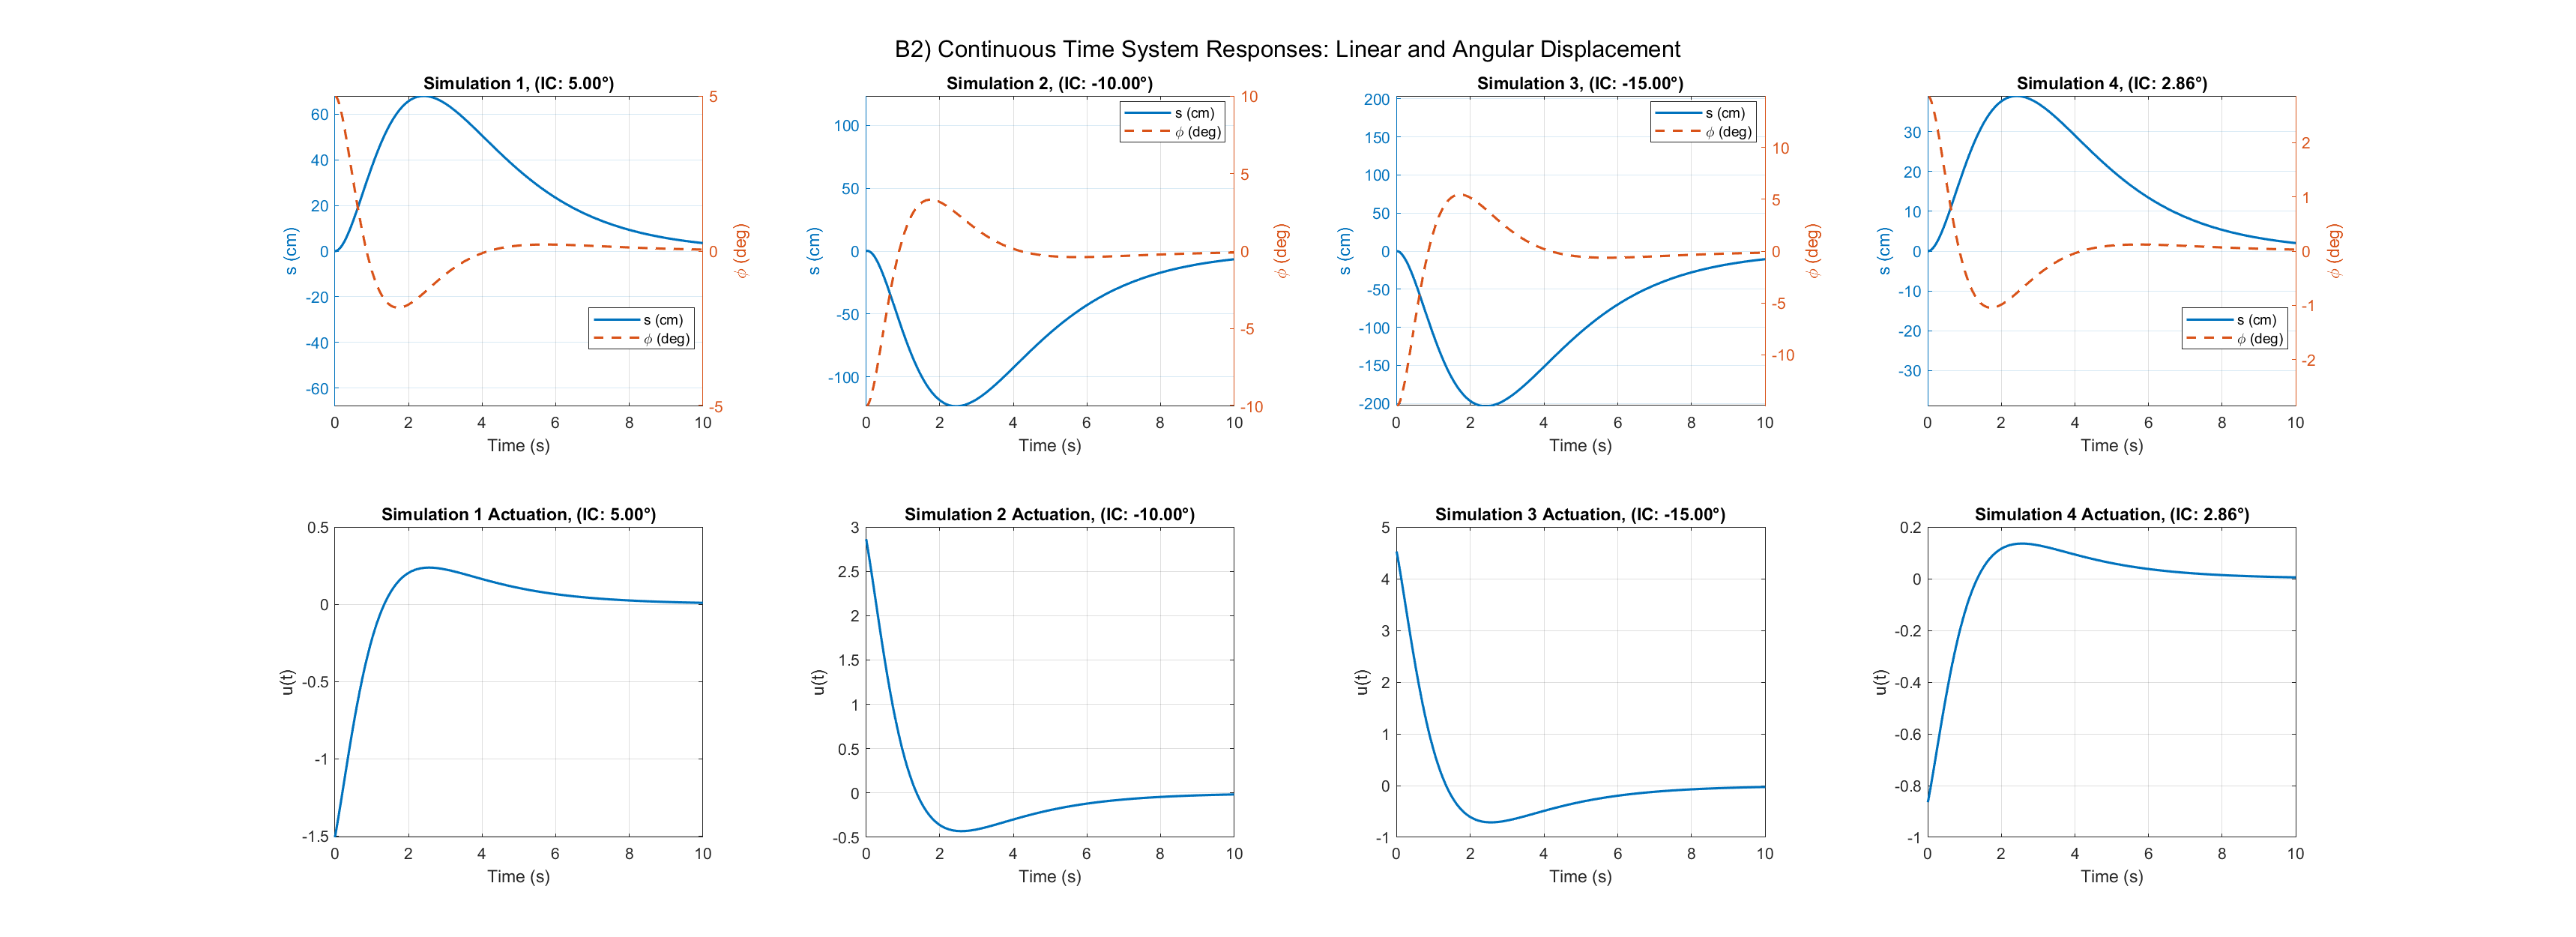
\includegraphics[width=20cm]{figures/b2.png}
    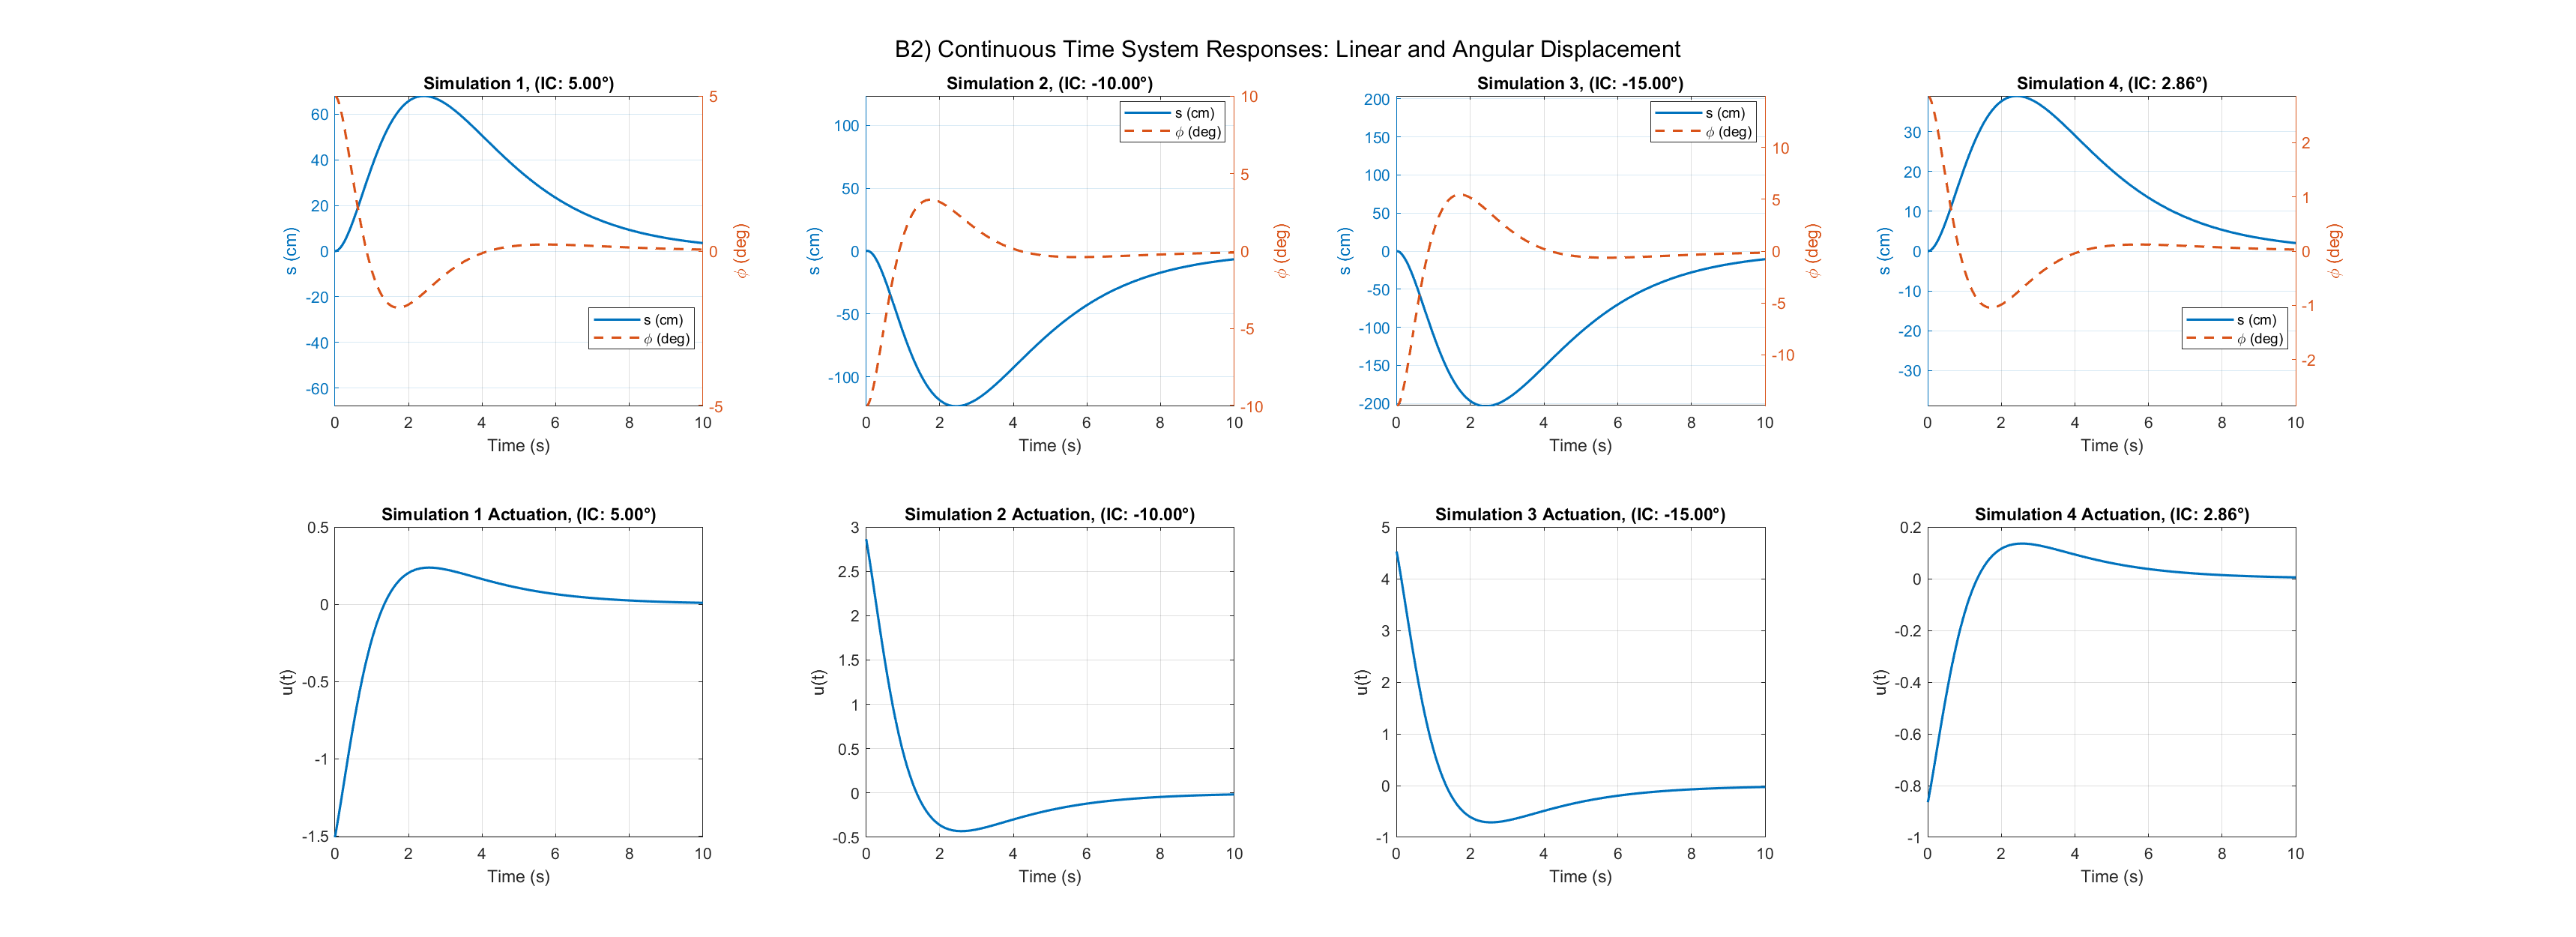
\includegraphics[width=\textwidth]{figures/b2.png}
    \caption{B2) Continuous Time System Responses: Linear and Angular Displacement}
    \label{b2}
\end{figure}

As shown, controller performance is incredibly strong, with the angular rate converging within 5 seconds across all trials with no overshoot or static error. The cart position converges more slowly compared to the pendulum, however, this is not prioritized because the objective is to keep the pendulum upright, not navigate the cart to $s=0$. The maximum experienced velocity of the carts across all simulations is $-1.2m/s$, which was deemed within the allowable values, especially when considering that this is when the starting angle was far from the equilibrium position the system was linearized around. 

\subsection*{B3) Nonlinear Simulation with a Linear Controller}
The same controller was simulated, however this time using the nonlinear differential equation derived in A1. The results are shown below in Figure \ref{B3}.

\begin{figure}[H]
    \centering
    % 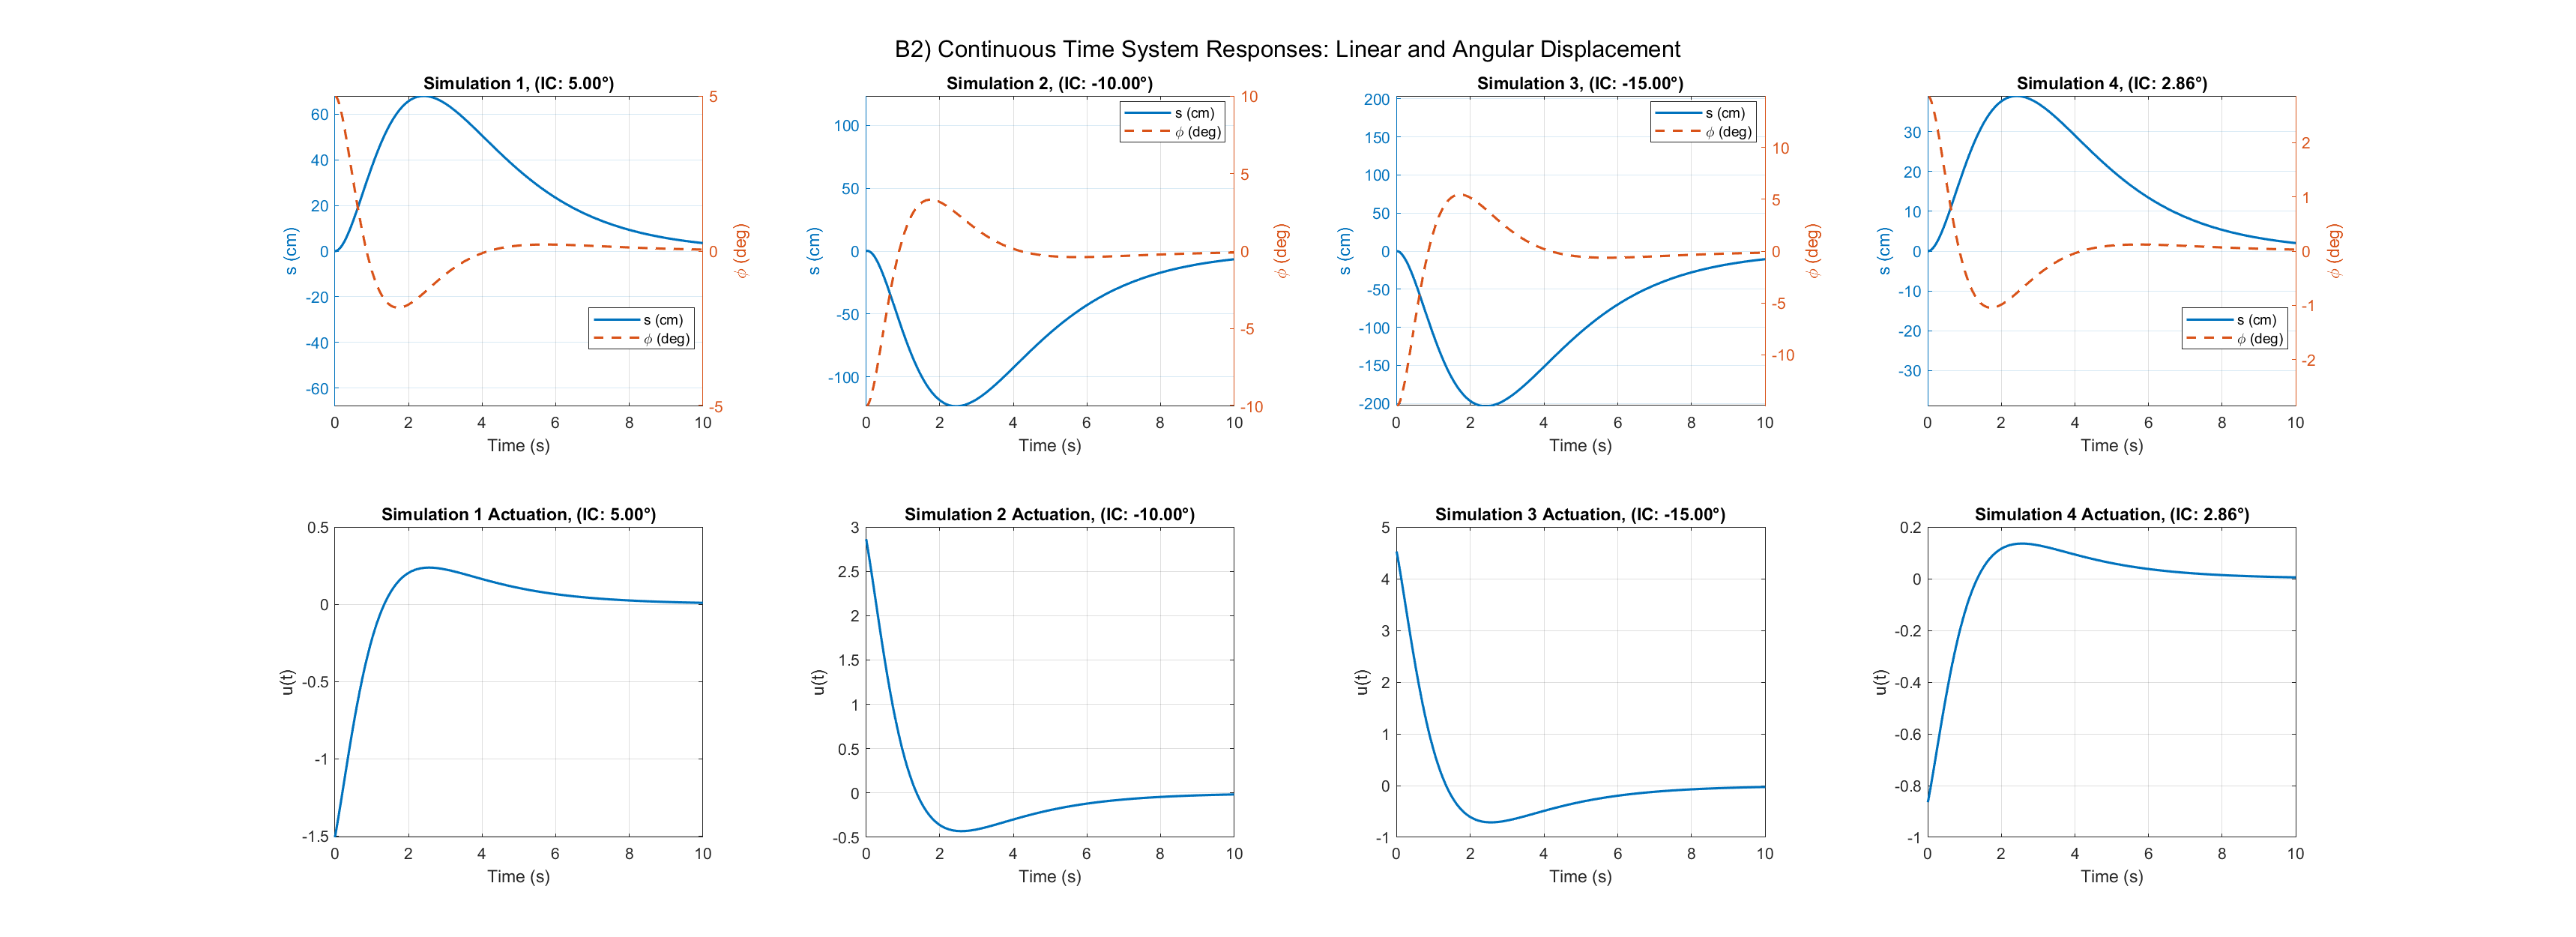
\includegraphics[width=20cm]{figures/b2.png}
    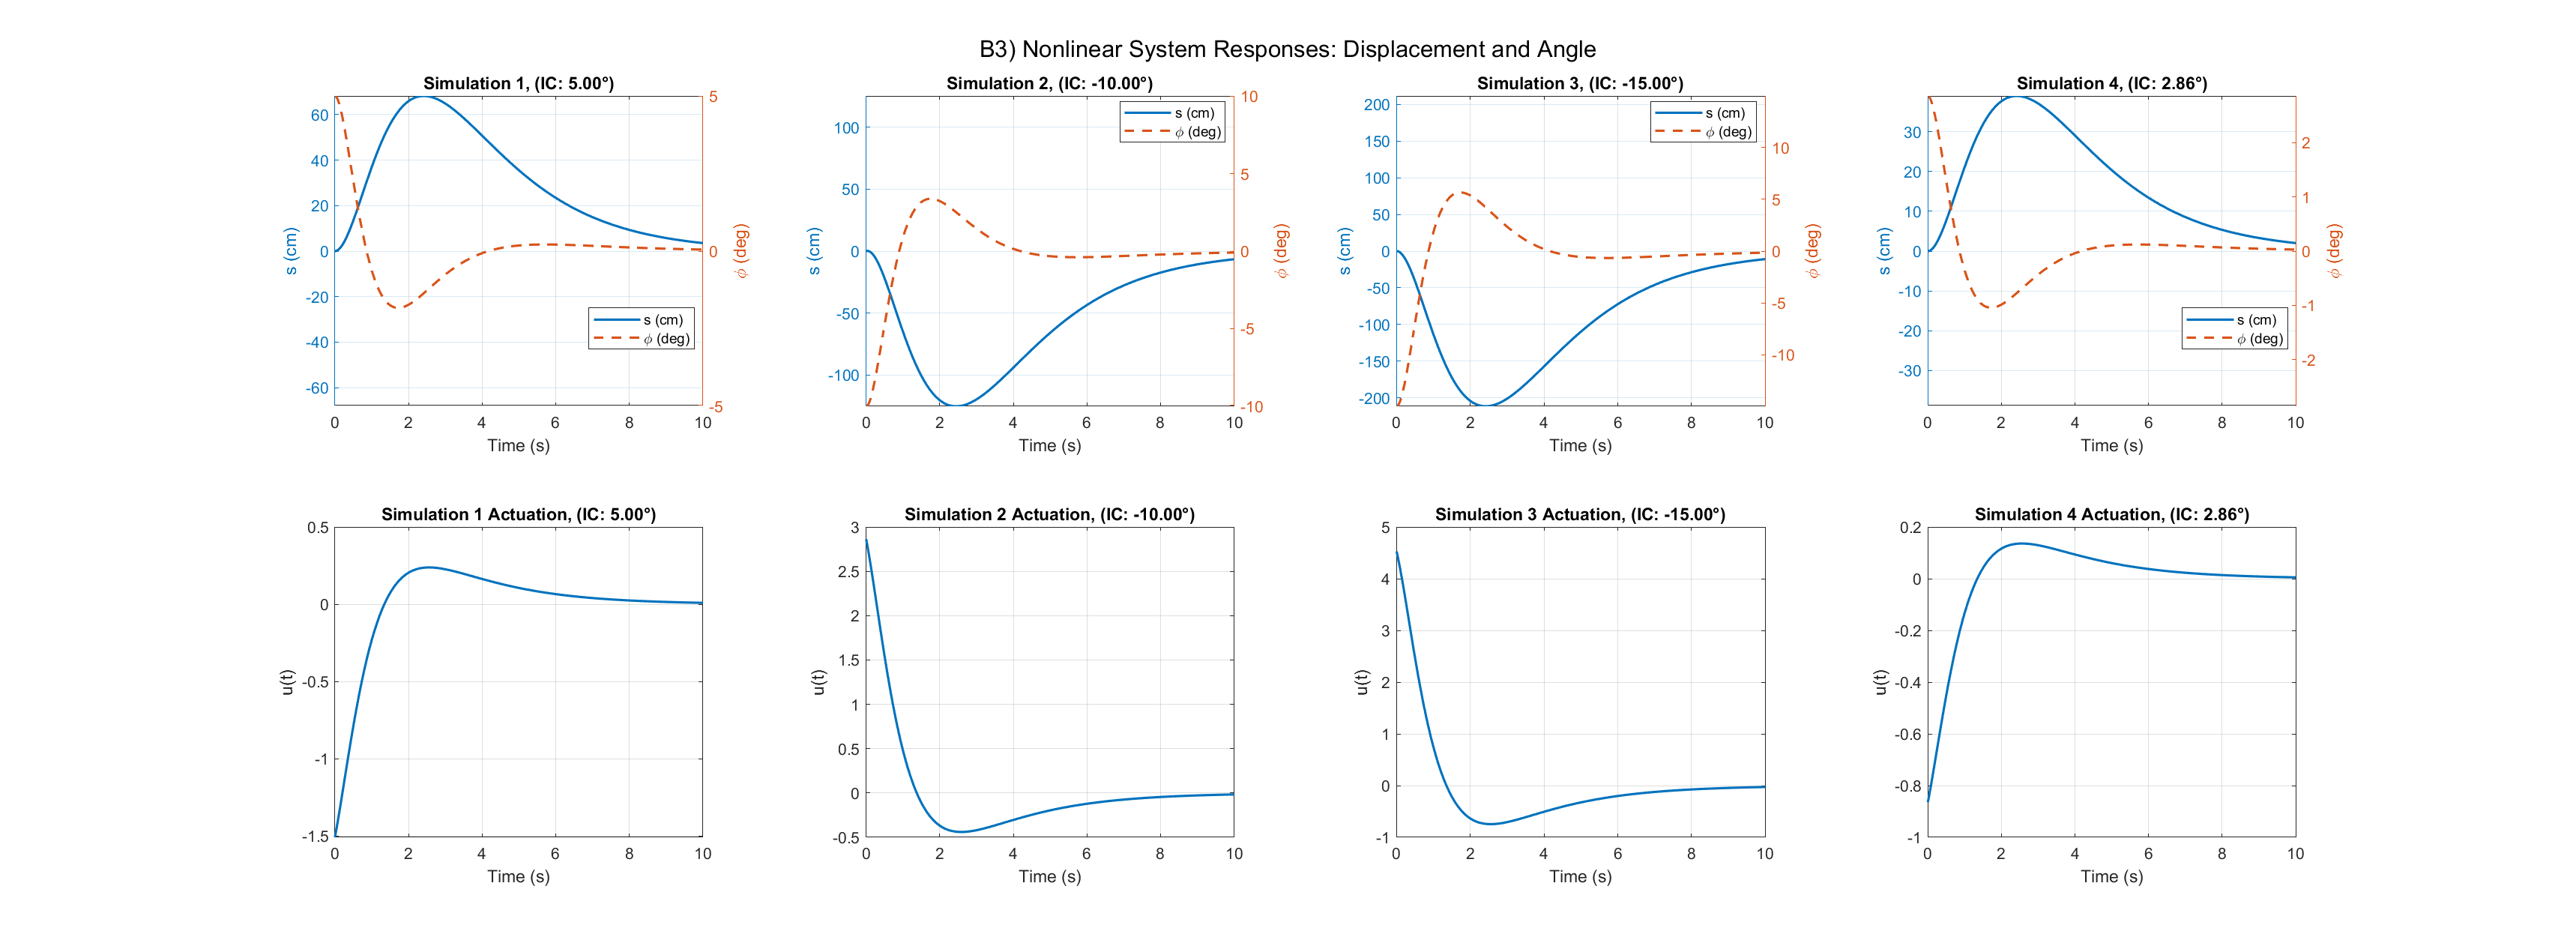
\includegraphics[width=\textwidth]{figures/b3_x.png}
    \caption{B3) Nonlinear System Responses: Displacement and Angle}
    \label{B3}
\end{figure}

The output of the two state responses are similar; however, in instances where the initial condition deviates far from the point the system was linearized around (simulations 2 and 3), the controller actuates larger movements to try and control the pendulum. Overall, the performance of the controller is still strong across all simulations.

\subsection*{B4) Stable Sampling Time}

some text

\subsection*{B5) Performance Degradation Across Sampling Times}

some text

\subsection*{B6) Discrete Time State Space Representation}
Matrices $A$ and $B$ were calculated in Equations \ref{jacobian} and \ref{jB} respectively. Section B4 noted that the slowest possible sampling time for this system is 1.3707to guarantee asymptotic stability. To introduce a non-unity safety factor, a sampling time of 0.2 was chosen for all future simulations to ensure behavior is as expected from the theoretical derivations of the controller.

To create the discrete-time state-space representation of the cart-pendulum system, the following definitions are used to write the system as $\dot x[k+1]=A_dx[k]+B_du[k]$. Equations \ref{ad} and \ref{bd} show the creation of matrices $A_d$ and $B_d$.

\begin{equation}\label{ad}
    A_d=e^{\n\left(\begin{array}{cccc} 0 & 1 & 0 & 0\\ 0 & -\frac{F}{M} & 0 & 0\\ 0 & 0 & 0 & 1\\ 0 & \frac{F}{LM} & \frac{g}{L} & 0 \end{array}\right)
\n*Ts}=
\end{equation}


\begin{equation}\label{Bd}
    B_d=1
\end{equation}

It is noted that $C_d=C$ and $D_d=D$ as these matrices do not introduce any new dynamics to the system.


\end{document}

